\documentclass[12pt]{report}
\usepackage[left=2.5cm,right=2.5cm,top=3cm,bottom=3cm]{geometry}
\usepackage{fancyhdr}
\usepackage{etoolbox}
\usepackage{titlesec}
\usepackage{titling} % para personalizar el título
\usepackage{amssymb}
\usepackage{amsmath}
\usepackage{graphicx}
\usepackage{ulem}
\usepackage{cancel}

\pagestyle{fancy}
\fancyhf{} 
\fancyhead[L]{UTN-FRC}
\fancyhead[C]{ASyS}
\fancyhead[R]{2R3}
\renewcommand{\headrulewidth}{0.4pt}
\fancyfoot[C]{\vfill\thepage}

\patchcmd{\chapter}{\thispagestyle{plain}}{\thispagestyle{fancy}}{}{}

\renewcommand{\chaptername}{Ejercicio}

\titleformat{\chapter}[display]
  {\normalfont\bfseries}{\chaptertitlename\ \thechapter}{15pt}{}
\titlespacing*{\chapter}{0pt}{0pt}{0pt}

\DeclareMathSizes{15}{13}{8}{8}

\setlength{\parskip}{6pt}

\title{%
  \fontsize{25}{0}\selectfont Universidad Tecnológica Nacional \\
  \fontsize{22}{30}\selectfont Analisis de Señales y Sistemas \\
  \fontsize{20}{25}\selectfont Trabajo Practico 1
}
\author{Luciano Cortesini}
\date{06 / 05 / 2024}

\begin{document}
\maketitle

\chapter{}%ejercicio 1
Considerar la ecuación en variable compleja $z^7-jz^7+2^{14}2e^{\frac{j\pi}{2}}=0$
Obtener el conjunto $S$ de números complejos que solucionan la ecuación

\textbf{a) Demostrar que  $S = \{z_k = 4e^{j(\frac{\pi}{4}+\frac{2k\pi}{7})} \mid k=-3;-2;-1;0;1;2;3\}$}\\

Resolucion:\\
\begin{align*}
&z^7 - jz^7 + 2^{14}\sqrt{2}e^{\frac{j\pi}{2}} = 0\\
&z^7(1-j) = 2^{14}\sqrt{2}e^{\frac{-j\pi}{2}}\\
&z^7 = \frac{2^{14}\sqrt{2}e^{-\frac{j\pi}{2}}} {2e^{-\frac{j\pi}{4}}}\\
&z = (2^{14}e^{j(-\frac{\pi} {4})})^{\frac{1}{7}}\\
&z = 4e^{j\frac{(-\frac{\pi}{4}+2k\pi)}{7}} \quad,\quad k = \{-3,-2,-1,0,1,2,3\}\\
\end{align*}

\textbf{b) Obtener el gráfico de normas del conjunto $S$, esto es:}
    $$k, |k| \quad | \quad k = -3;-2;-1;0;1;2;3 $$
Resolucion:\\
\begin{figure}[h] % Aquí comienza el ambiente de figura
    \centering % Centrar la imagen
    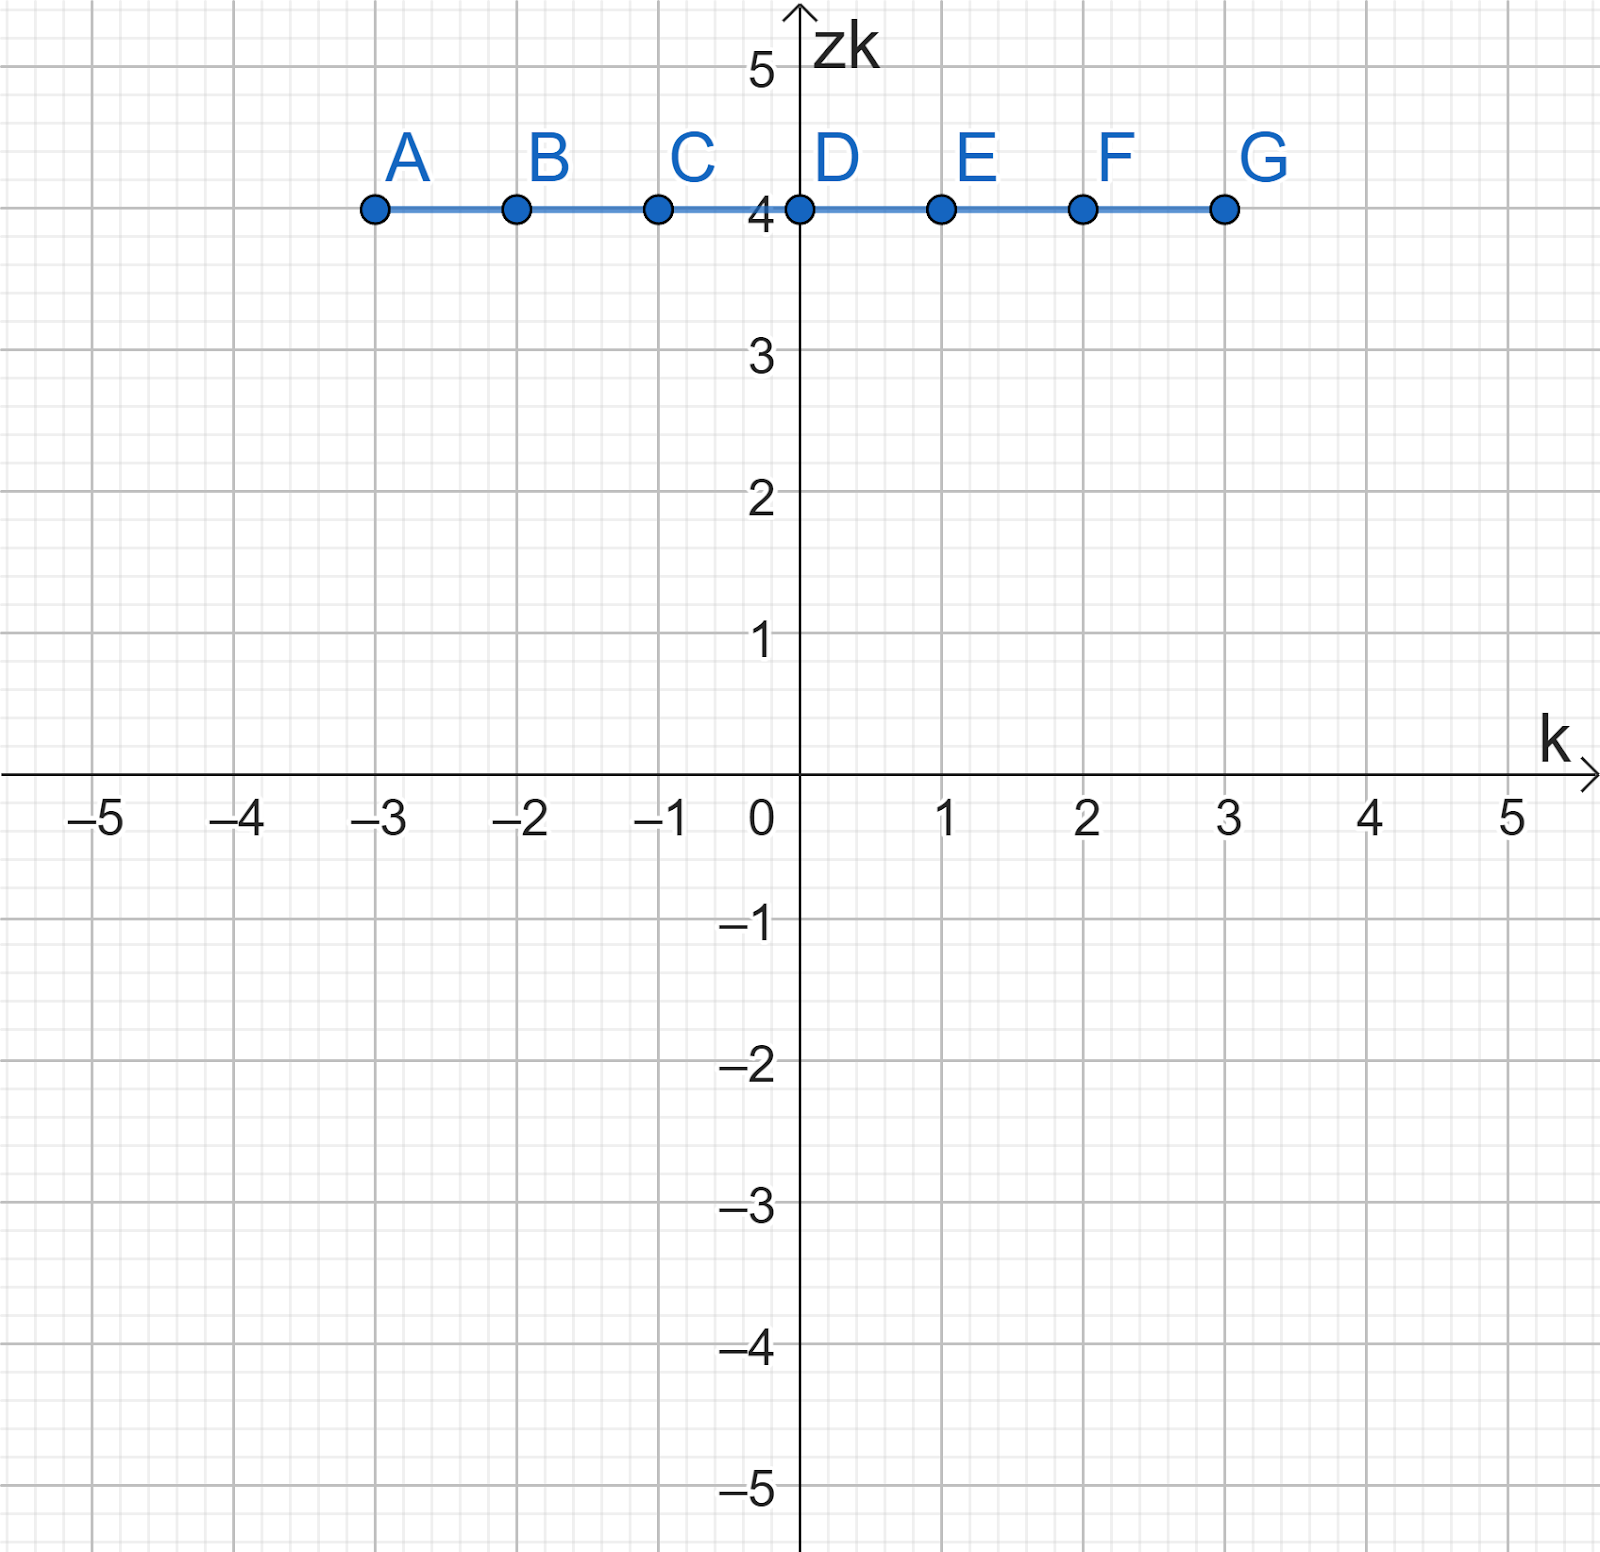
\includegraphics[width=0.4\textwidth]{./Imagenes/foto1Ej1.png} % Insertar la imagen
\end{figure}

\textbf{c) Obtener el gráfico de argumentos principales del conjunto $S$, esto es:}
    $$k, Arg(z_k) \quad | \quad k = -3;-2;-1;0;1;2;3 $$
Resolucion:\\
\begin{figure}[h] % Aquí comienza el ambiente de figura
    \centering % Centrar la imagen
    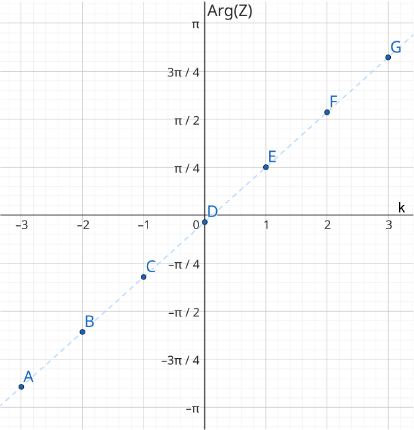
\includegraphics[width=0.4\textwidth]{./Imagenes/foto2Ej1.png} % Insertar la imagen
\end{figure}
\chapter{}%ejercicio 2
Considerar las siguientes funciones de variable compleja $z = x + jy$:
$$f_1(z) = (4y - y^2 - x - \frac{1}{3}y^3) - j(y + 2x^2 + \frac{1}{3}x^3)$$
$$f_2(z) = (4z - z^2 - z - \frac{1}{3}z^3) - j(z + 2z^2 + \frac{1}{3}z^3)$$

\textbf{a) Obtener la parte real $u_1 = \text{Re}(f_1)$ y la parte imaginaria $v_1 = \text{Im}(f_1)$
, y exponer la igualdad $f_1(z) = u_1 + jv_1$. Similarmente, para la función $f_2(z)$.}\\

$f_1$ parte real e imaginaria
$$U_1=Re(f_1)=4y-y^2-x-\frac{1}{3}y^3$$
$$V_1=Im(f_1)=-y-2x^2-\frac{1}{3}y^3$$

Para obtener la parte real e imaginaria de $f2$, reemplazamos $z=x+jy$\\
Para el primer termino:
$$4z - z^2 - z - \frac{1}{3}z^3=(x+jy) - (x+jy)^2 - (x+jy) - \frac{1}{3}(x+jy)^3$$
$$=4x + 4jy -x^2 -2xyj + y^2 -x -jy - \frac{1}{3}x^3 - jx^2y + xy^2 + \frac{1}{3}jy^3$$
$$=(- \frac{1}{3}x^3 -x^2 + 3x + y^2 + xy^2) +j(3y -2xy + \frac{1}{3}y^3 - x^2y )$$ \\
Para el segundo termino:
$$-j (z + 2z^2 + \frac{1}{3}z^3) = -j ((x+jy) + 2(x+jy)^2 + \frac{1}{3}(x+jy)^3)$$
$$=-j (x+jy + 2(x^2+2xyj-y^2) + \frac{1}{3}(x^3 + 3x^2yj + 3x(yj)^2 + (jy)^3))$$
$$=-j ((x + 2x^2 - 2y^2 + \frac{1}{3} x^3 - xy^2) + j( y +4xy + x^2y - \frac{1}{3}y^3))$$
$$=j(-x - 2x^2 + 2y^2 - \frac{1}{3} x^3 + xy^2) + ( y +4xy + x^2y - \frac{1}{3}y^3)$$\\
Luego de separar ambos terminos de $f_2$ en su parte real e imaginaria encontraremos la parte real
e imaginaria de $f_2$
$$U_2=Re(f_2)=- \frac{1}{3}x^3 - x^2 + 3x + y^2 + xy^2 + y +4xy + x^2y - \frac{1}{3}y^3$$
$$V_2=Im(f_2)=-x + 3y -2xy - 2x^2 + 2y^2 - x^2y + xy^2 + \frac{1}{3}y^3 - \frac{1}{3} x^3$$

\textbf{b) Obtener el conjunto de números complejos $D_1$ donde la función $f_1(z)$ es derivable. Similarmente, obtener $D_2$ donde $f_2(z)$ es derivable.
¿Hace falta resolver las ecuaciones de Cauchy-Riemann para determinar $D_2$?}

Para obtener el conjunto de numeros complejos $D_1$ donde la funcion $f_1(z)$ es derivable, utilizaremos las ecuaciones de Cauchy-Riemman
$$\frac{\delta U_1}{\delta x}=-1 \quad \quad \frac{\delta V_1}{\delta x}=-4x-x^2$$
$$\frac{\delta V_1}{\delta y}=-1 \quad \quad - \frac{\delta U_1}{\delta y}=-(4-2y-y^2)=y^2+2y-4$$
si:$$\frac{\delta V_1}{\delta x}=-\frac{\delta U_1}{\delta y}$$
$$-4x-x^2=y^2+2y-4$$
$$x^2+4x+y^2+2y=4$$
$$(x+2)^2+(y+1)^2=9$$\\
Entonces, el conjunto de numeros complejos $D_1$ donde $f_1$ es derivable es:
$$D_1 = \{z \in \mathbb{C} : |z + 2 + j| = 3\}$$

Para obtener el conjunto de numeros complejos $D_2$ donde $f_2$ es derivable, no es necesario aplicar las ecuaciones de Cauchy-Riemman,
ya que la funcion es un polinomio complejo, por lo tanto:
$$D_2=\mathbb{C}$$\\

\textbf{c) Demostrar que $D_1 = \{z \in \mathbb{C} : |z + 2 + j| = 3\}$ y $D_2 = \mathbb{C}$.}

$$|z+2+j|=3$$
$$|(x+jy)+2+j|=3$$
$$|x+2+j(y+1)|=3$$
$$\sqrt{(x+2)^2+(y+1)^2}=3$$
$$(x+2)^2+(y+1)^2=3^2$$\\

\textbf{d) Demostrar que la función $f_1(z)$ no es analítica y que la función $f_2(z)$ es entera.}

Al ver los resultados obtenidos por Cauchy-Riemann, observamos que las derivadas parciales de $f1$ nos dan una condición, en este caso $f1$ es derivable solamente
en $D1 = \{z \in \mathbb{C} : |z + 2 + j| = 3\}$, o sea una circunferencia de radio $3$ centrada en $(-2, -j)$, sin embargo para cualquier punto de $f$ en la
circunferencia no hay una vecindad o disco abierto alrededor del punto en cuestión en el que se satisfagan las ecuaciones de Cauchy-Riemann.

$f2$ es una función compleja cuyo dominio abarca todo el plano complejo. Dado que $f2$ es una composición de polinomios, se garantiza la continuidad y
derivabilidad en todo su dominio. Además, al ser derivable en cada punto del plano complejo, $f2$ es analítica en cada punto del dominio, cumpliendo las
condiciones necesarias para decir que la $f2$ es una función entera

\textbf{e) De las funciones anteriores, ¿se puede afirmar que "Derivable implica analítica" o "Analítica implica derivable"? ¿Por qué?}

La analiticidad no implica derivabilidad, porque, para que una función sea analítica no basta con ser derivable en un punto sino en todo el dominio de esa
función, cumpliendo así también con las ecuaciones de Cauchy-Riemann.\\

\textbf{f) De las funciones anteriores, ¿se puede afirmar que $f'_1(z) = u_{1x} + jv_{1x}$ o $f'_2(z) = u_{2x} + jv_{2x}$? ¿Por qué?}
Se puede afirmar que:

$$f'_1(z)=\frac{\delta U_1}{\delta x}+\frac{\delta V_1}{\delta x}$$
$$f'_2(z)=\frac{\delta U_2}{\delta x}+\frac{\delta V_2}{\delta x}$$

porque tanto la $f1$ y la $f2$, cumplen Cauchy-Riemann y en particular, $f2$ es una función entera, entonces se puede decir en este caso que las derivadas de las
funciones son iguales a las derivadas parciales de $u$ y $v$ con respecto a $x$ e $y$

\chapter{}%ejercicio 3

Considerar $$ f(z) = w $$ el mapeo bilineal que transforma los puntos:

\begin{align*}
    z_1 &= \infty, \quad & w_1 &= -j \\
    z_2 &= -j, \quad & w_2 &= 0 \\
    z_3 &= 0, \quad & w_3 &= \infty 
\end{align*}

\textbf{a) Desarrollar la fórmula que determina al mapeo \( f(z) \), empleando razones cruzadas.}

Resolución: Se procede partiendo desde la definición de mapeo para una razón cruzada:

$$ \frac{z - z_1}{z - z_3} \cdot \frac{z_2 - z_3}{z_2 - z_1} = \frac{w - w_1}{w - w_3} \cdot \frac{w_2 - w_3}{w_2 - w_1} $$

Antes de reemplazar los valores de los puntos en la definición anterior, es más cómodo si se simplifica acorde al ejercicio. Debido a que tenemos puntos que tienden al infinito en ambos \( w \) y \( z \), vamos a sacar factor común de aquellos puntos, con el objetivo de simplificarlos, ya sea por cancelación o utilizando las identidades de los números hiperreales:

\begin{align*}
    \frac{z_1 \left(\frac{z}{z_1}-1\right) }{z-z_3} \frac{z_2-z_3}{z_1 \left( \frac{z_3}{z_2} -1 \right) } &= \frac{w-w_1}{w_3 \left( \frac{w}{w_3} - 1 \right)} \frac{w_3 \left( \frac{w_1}{w_3} -1 \right) }{w_2-w_1}\\[10pt]
    \frac{\frac{z}{z_1} -1}{z-z_3} \frac{z_2-z_3}{\frac{z_3}{z_1}-1} &= \frac{w-w_1}{\frac{w}{w_3}-1} \frac{\frac{w_1}{w_3}-1}{w_2-w_1}\\
\end{align*}
Ahora si, reemplazando los puntos:\\

$$\frac{\frac{z}{\infty}-1}{z-0} \frac{-j-0}{\frac{0}{\infty}-1} = \frac{w-(-j)}{\frac{w}{\infty}-1} \frac{\frac{-j}{\infty}-1}{0-(-j)}$$\\

Por las identidades de los números hiperreales, cualquier número dividido una magnitud infinita es igual a cero:\\

\begin{align*}
    \frac{0-1}{z} \frac{-j}{0-1} &= \frac{w+j}{0-1} \frac{0-1}{j}\\
    \frac{-1}{z} \frac{-j}{-1} &= \frac{w+j}{-1} \frac{-1}{j}\\
    \frac{-1}{z}j &= (-w-j)j\\
    -\frac{1}{z}+j &= -w\\
    w &= \frac{1}{z}-j\\
\end{align*}

\textbf{b) Obtener las fórmulas y graficar \( R' \) en el plano \( W \), sabiendo que \( R = \{z \in \mathbb{C} \mid \text{Im}(z) - 2\text{Re}(z) = 0\} \) en el plano \( W \).}

Resolución: Para simplificar el desarrollo del ejercicio, se realizarán dos mapeos. Uno, \( w_0 \), que va a ser el mapeo recíproco, y otro, \( w_1 \), que va a ser la traslación del mapeo \( w_0 \) a \( -j \).

Para empezar, necesitamos encontrar la relación que tienen las componentes \( x \) e \( y \) (de \( z \)) respecto de \( u \) y \( v \) (de \( w_0 \)):

\begin{align*}
    w_0 &=\frac{1}{z}\\
    u+jv &=\frac{1}{x+jy}\\
    x+jy &= \frac{1}{u+jv}\\
    x+jy &= \frac{1}{u+jv} \frac{u-jv}{u-jv}\\
    x+jy &= \frac{u-jv}{u^2+juv-juv-j^2y^2}\\
    x+jy &= \frac{u}{u^2+v^2}-j\frac{v}{u^2+v^2}\\
    x=\frac{u}{u^2+v^2} \hspace{0.5cm} &;\hspace{0.5cm} y=-\frac{v}{u^2+v^2}\\
\end{align*}
Ya teniendo las relaciones entre \( w_0 \) y \( z \), procedemos a operar la ecuación que define el conjunto, y reemplazar con sus respectivas igualdades las variables que correspondan:

\begin{align*}
&\text{Im}(z) - 2\text{Re}(z) = 0\\ 
&y - 2x = 0\\ 
&-\frac{v}{u^2 + v^2} - 2\frac{u}{u^2 + v^2} = 0\\ 
&-\frac{v}{u^2 + v^2} = 2\frac{u}{u^2 + v^2}\\ 
&-v=2u\\
&-v - 2u = 0\\ 
&-v - 2u = w_0\\ 
\end{align*}

Ya teniendo \( w_0 \), para completar el mapeo, es tan simple como reemplazar el resultado obtenido en \( w_1 \), y se obtiene la ecuación que define el nuevo conjunto \( R' \):

$$ w_1 = w_0 - j $$
$$ w_1 = -v - 2u - j $$
$$ R' = \{w \in \mathbb{C} \mid -v - 2u = j\} $$

\begin{figure}[h] % Aquí comienza el ambiente de figura
    \centering % Centrar la imagen
    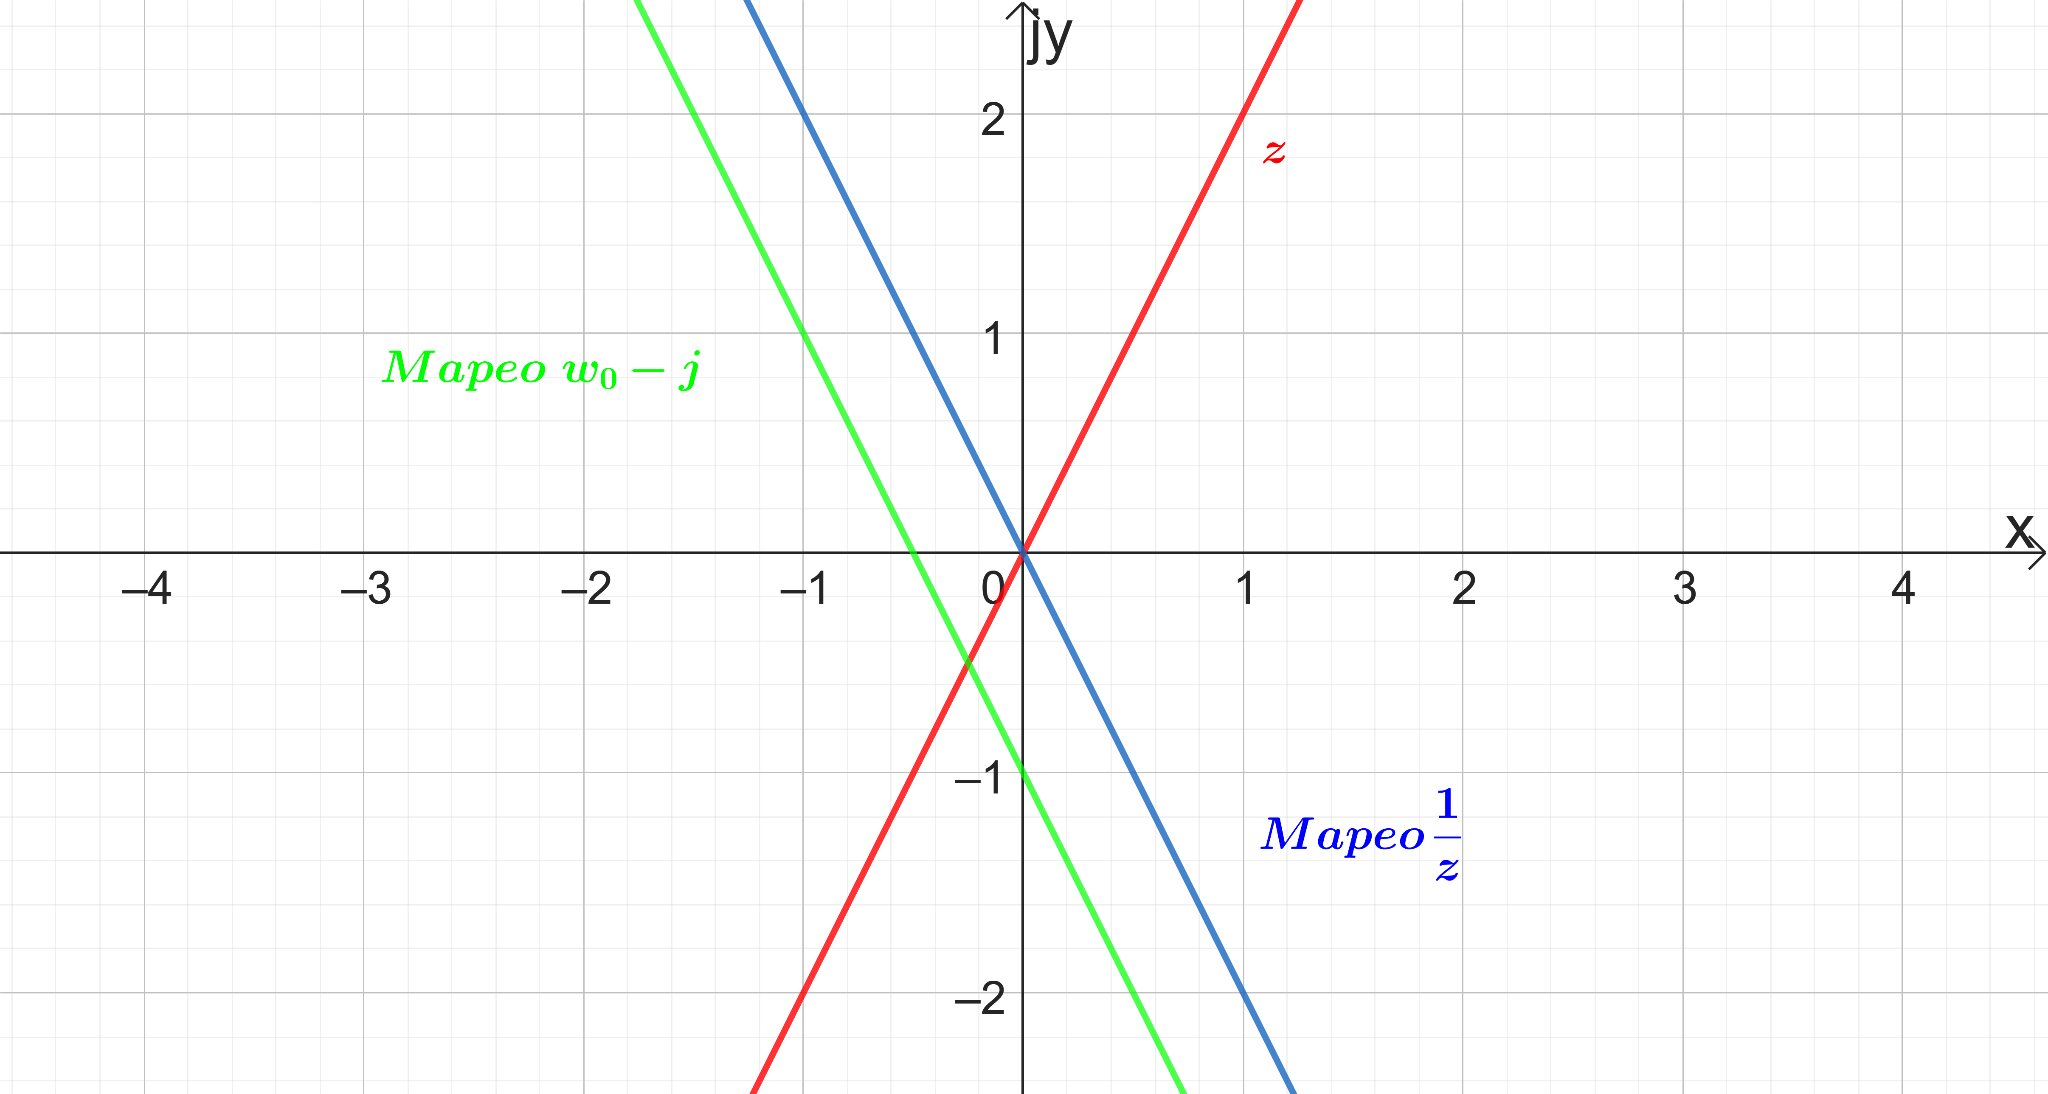
\includegraphics[width=0.65\textwidth]{./Imagenes/foto1Ej3.png} % Insertar la imagen
\end{figure}

\textbf{c) Obtener las fórmulas y graficar \( C' \) en el plano \( W \), sabiendo que \( C = \{z \in \mathbb{C} \mid |z - 1 - j| = 2\} \) en el plano \( W \).}\\[6pt]

Resolución: Para simplificar el desarrollo del ejercicio, como se hizo antes, se realizarán dos mapeos. Uno, \( w_0 \), que va a ser el mapeo recíproco, y otro, \( w_1 \), que va a ser la traslación del mapeo \( w_0 \) a \( -j \).

Para no repetir, vamos a traer del punto b, las relaciones de \( x \) e \( y \) (de \( z \)) respecto de \( u \) y \( v \) (de \( w_0 \)):

$$ x = \frac{u}{u^2 + v^2}, \quad y = \frac{-v}{u^2 + v^2} $$\\[6pt]
Ahora simplemente obtenemos la ecuación que define el conjunto y reemplazamos correspondientemente:\\
\begin{align*}
|z-1-j| &= 2 \\[6pt]
|x+jy-1-j|  &= 2 \\[6pt]
|x-1+jy-j| &= 2 \\[6pt]
|(x-1)+j(y-1)| &= 2 \\[6pt]
  \sqrt{(x-1)^2 + (y-1)^2} &= 2 \\[6pt]
(x-1)^2 + (y-1)^2 &= 2 \\[6pt]
x^2 - 2x + 1 + y^2 - 2y + 1 &= 2 \\[6pt]
x^2 - 2x + y^2 - 2y + 2 &= 2 \\[6pt]
x^2 - 2x + y^2 - 2y &= 0 \\[6pt]
   \left(\frac{u}{u^2+v^2} \right)^2 - 2\frac{u}{u^2+v^2} + \left( -\frac{v}{u^2+v^2} \right)^2-2 \left( -\frac{v}{u^2+v^2} \right) &=0\\[6pt]
   \frac{u^2}{(u^2+v^2)^2}-2\frac{u}{u^2+v^2} + \frac{v^2}{(u^2+v^2)^2}+2\frac{v}{u^2+v^2}&=0\\[6pt]
\frac{u^2}{(u^2+v^2)^2}+\frac{v^2}{(u^2+v^2)^2}&=2\frac{u}{u^2+v^2} - 2 \frac{v}{u^2+v^2}\\[6pt]
   \frac{1}{u^2+v^2} \left( \frac{u^2}{u^2+v^2} + \frac{v^2}{u^2+v^2} \right) &= \frac{1}{u^2+v^2}(2u-2v)\\[6pt]
   \frac{u^2+v^2}{u^2+v^2}&=2u-2v\\[6pt]
\end{align*}
\begin{align*}
     1 &= 2u - 2v \\[6pt]
    w_0 &= 2u - 2v - 1\\[6pt]
 \end{align*}
 
 Ya teniendo $w_0$, para completar el mapeo, es tan simple como reemplazar el resultado obtenido en $w_1$, y se obtiene la ecuación que define el nuevo conjunto \( C' \):\\
 
 
 \begin{align*}
     w_1 &= w_0-j \\[5pt]
     w_1 &= 2u-2v-1-j \\[5pt]
     C' &= \{w \in \mathbb{C} \, | \, 2u-2v-j=1\}
 \end{align*}
 
 
\begin{figure}[htbp] % Aquí comienza el ambiente de figura
    \centering % Centrar la imagen
    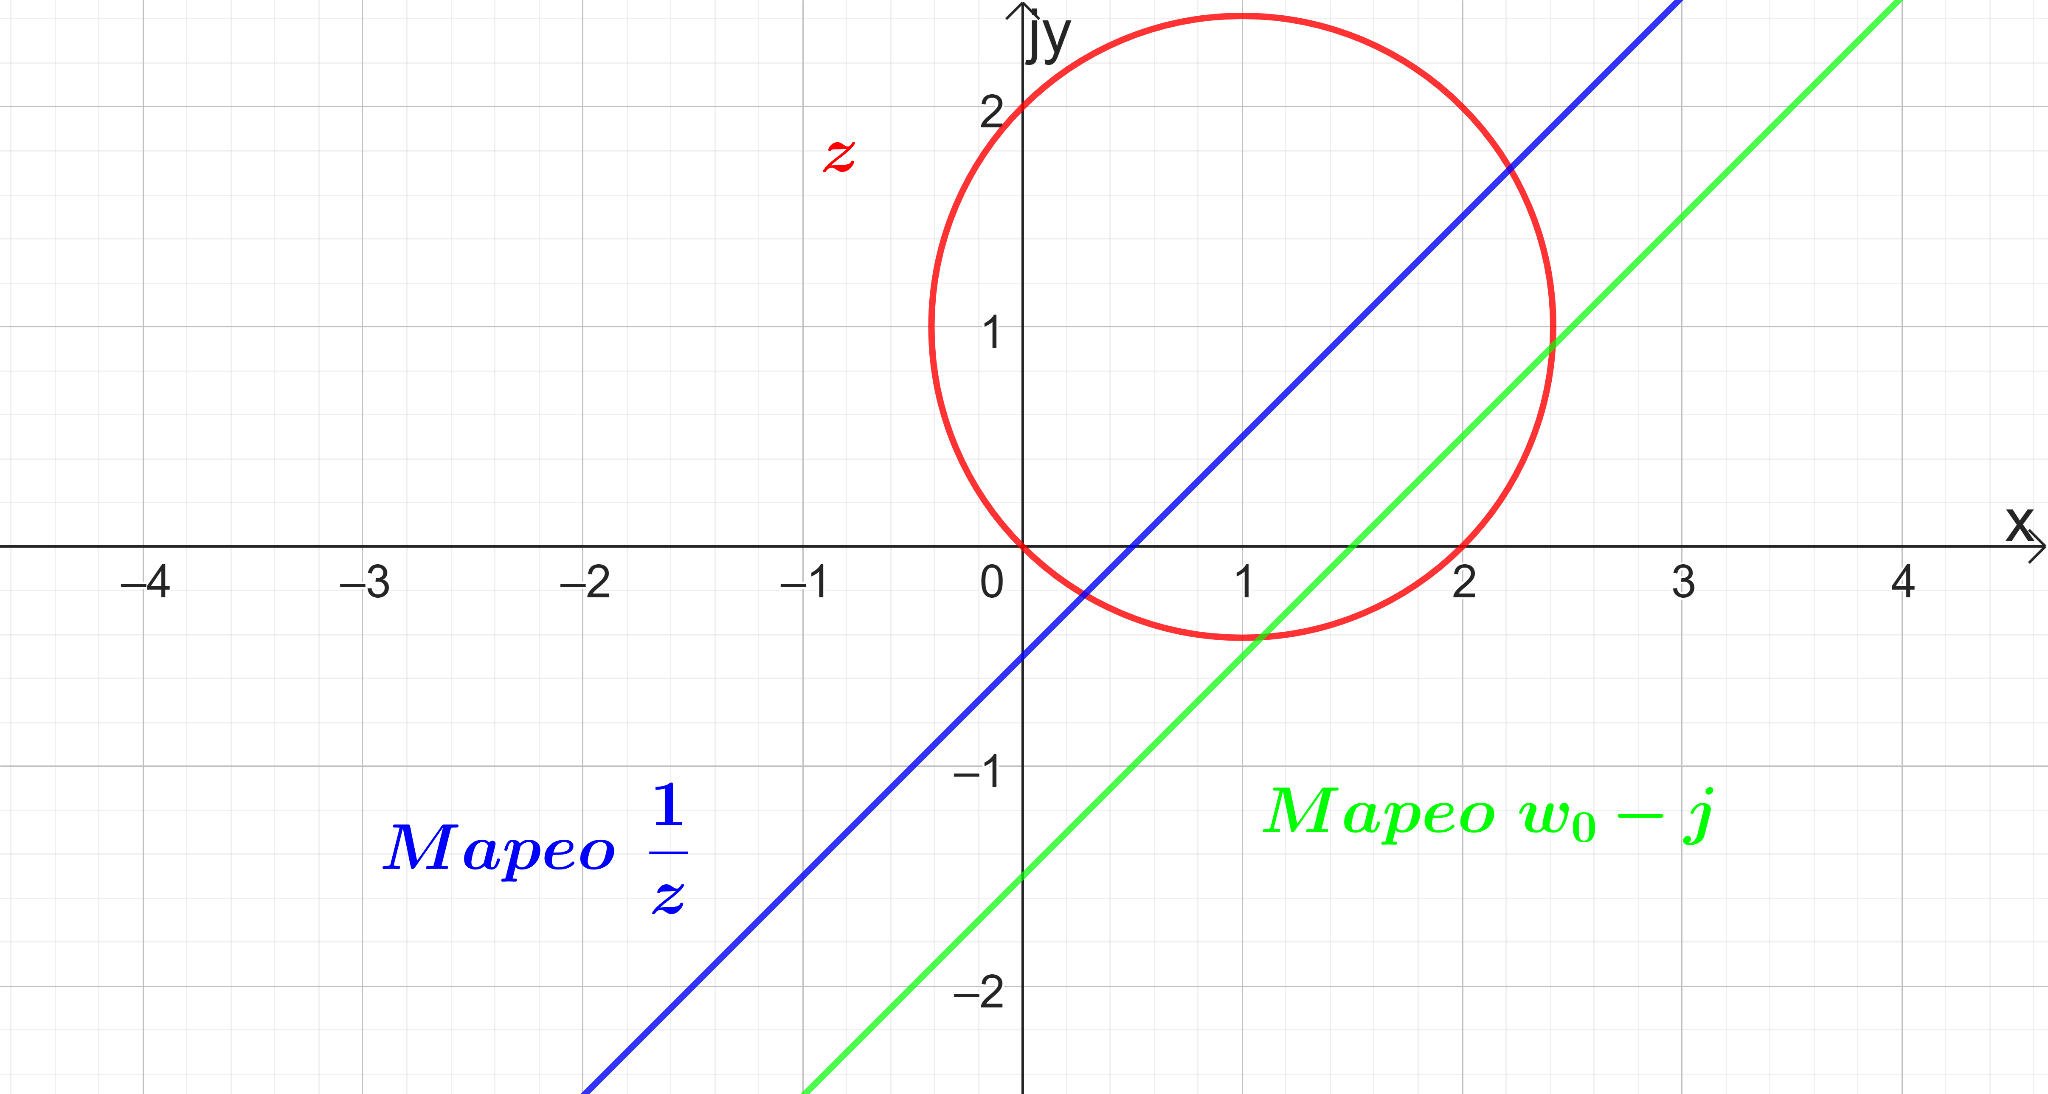
\includegraphics[width=0.65\textwidth]{./Imagenes/foto2Ej3.png} % Insertar la imagen
\end{figure}

\clearpage

\chapter{}%ejercicio 4

Con este ejercicio se espera que el estudiante controle el comportamiento de un mapeo expresándolo previamente como una composición de mapeos básicos, y como ello, obtener fácilmente las fórmulas de una región en el plano $W$ dadas las fórmulas en el plano $Z$. Considerar el mapeo $w = e^{3z + 2}$.

\textbf{a)} Graficar la región $R = \{z \in \mathbb{C} \, | \, 2 \leq \text{Re}(z) \leq 5; \frac{\pi}{4} \leq \text{Im}(z) \leq \frac{\pi}{2}\}$.

Resolucion:
Graficamos la región $R = \{z \in \mathbb{C} \, | \, 2 \leq \text{Re}(z) \leq 5; 4 \leq \text{Im}(z) \leq 2\}$ en el plano $Z$.

Parametrizando la frontera de $R$ en:
\begin{itemize}
    \item $R_1 = x + j4$, $2 \leq x \leq 5$
    \item $R_2 = 5 + jy$, $4 \leq y \leq 2$
    \item $R_3 = x + j2$, $2 \leq x \leq 5$
    \item $R_4 = 2 + jy$, $4 \leq y \leq 2$
\end{itemize}


\begin{figure}[h] % Aquí comienza el ambiente de figura
    \centering % Centrar la imagen
    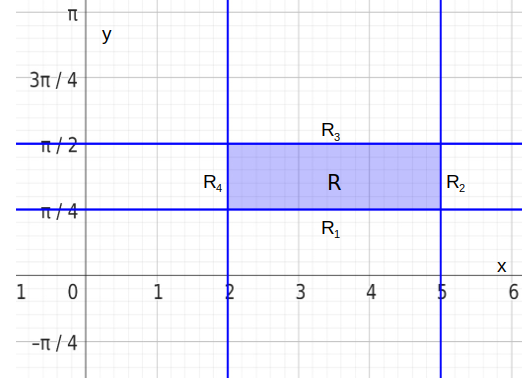
\includegraphics[width=0.65\textwidth]{./Imagenes/foto1Ej4.png} % Insertar la imagen
\end{figure}

\textbf{b)} Obtener las fórmulas y graficar $R' = \{w = f(z) \, | \, z \in R\}$ en el plano $W$, al ser mapeada desde $R$ en el plano $Z$.

Resolucion:
El mapeo dado se puede expresar como una combinación de tres mapeos:

\begin{itemize}
    \item $z \rightarrow 3z$ (ampliación)
    \item $z \rightarrow e^z$ (mapeo exponencial)
    \item $w \rightarrow w + 2$ (traslación)
\end{itemize}

Al aplicar los mapeos, obtenemos en un plano $w$ una región $R$, formada por dos rayos (mapeos de $R_1$ y $R_3$), y por dos arcos de circunferencia (mapeos de $R_2$ y $R_4$).

La nueva región $R'$ está parametrizada por:
\begin{itemize}
    \item $R_1 = e^{3x+j\frac{3\pi}{4}} + 2$, $2 \leq x \leq 5$
    \item $R_2 = e^{3 \cdot 5+j3y} + 2$, $4 \leq y \leq 2$
    \item $R_3 = e^{3x+j\frac{3\pi}{2}} + 2$, $2 \leq x \leq 5$
    \item $R_4 = e^{3 \cdot 5+j3y} + 2$, $4 \leq y \leq 2$
\end{itemize}


\begin{figure}[h] % Aquí comienza el ambiente de figura
    \centering % Centrar la imagen
    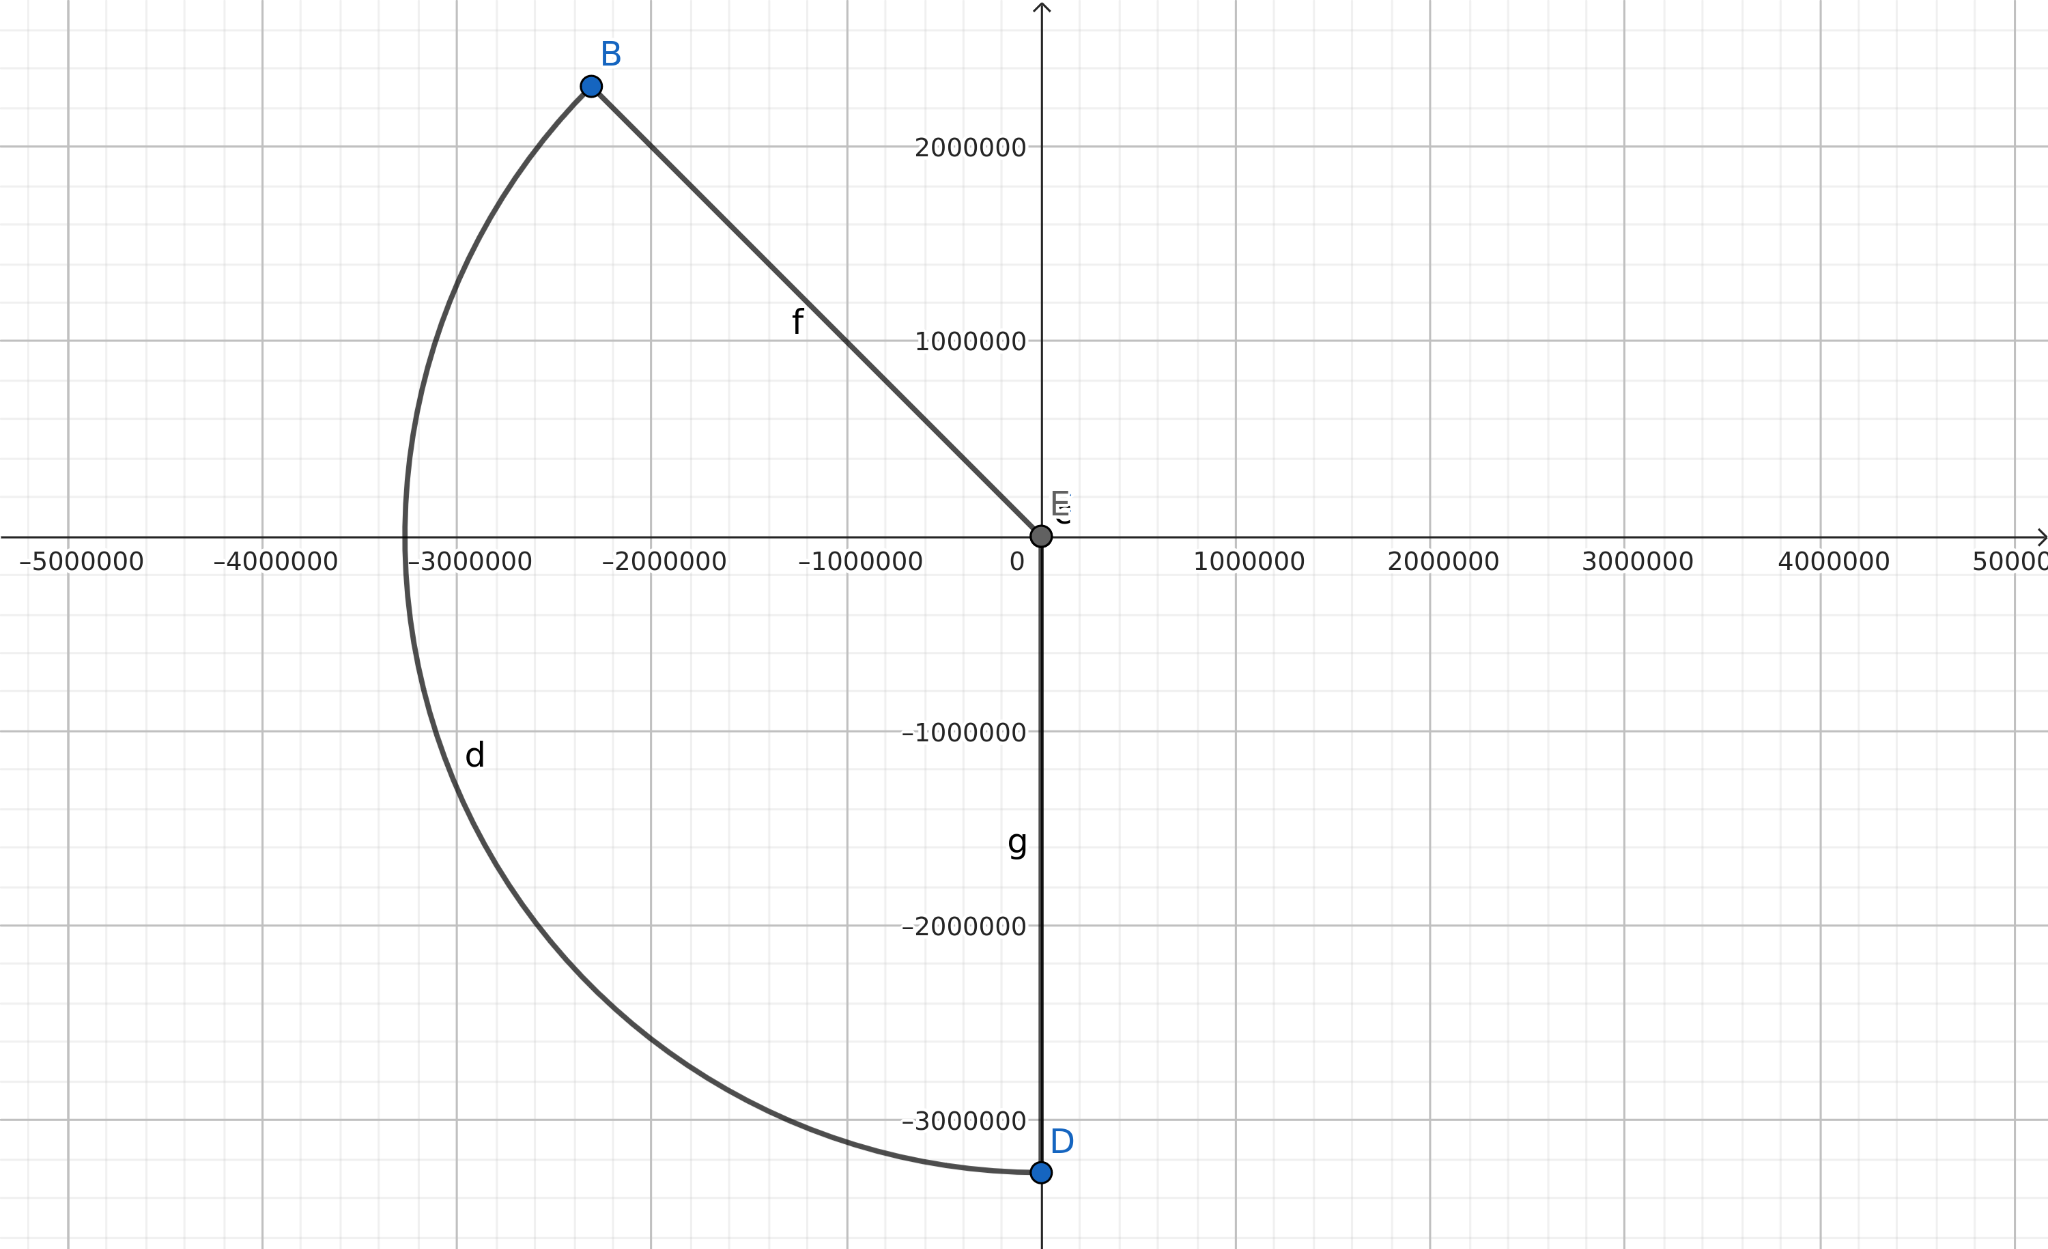
\includegraphics[width=0.65\textwidth]{./Imagenes/foto2Ej4.png} % Insertar la imagen
\end{figure}

\chapter{}%ejercicio 5

Considerar la función de variable compleja $f(z) =\frac{z + 3}{j(z - 1)^2(z^2 + 9)}$\\[6pt]

\textbf{a) Obtener el conjunto de ceros y el conjunto de singularidades de la función.}\\[6pt]

Ceros $\rightarrow f(z)=0$\\

\begin{align*}
&f(z)=\frac{z + 3}{j(z - 1)^2(z^2 + 9)}\\[6pt]
&z+3j=0\\[6pt]
&z=-3j\\[6pt]
\end{align*}
    
singularidades:\\

Como la funcion es un conciente de polinomios complejos va a tener singularidades cuando el denominador sea cero;\\

\begin{align*}
    &(z-1)^2(z^2+9)=0\\[6pt]
    &(z-1)^2=0 \hspace{3.5cm}    z^2+9=0\\[6pt]
    &z-1=0     \hspace{4cm}   z=\sqrt{-9}\\[6pt]
    &z=1       \hspace{4.75cm}  z=\pm3j\\[6pt]
\end{align*}

El conjunto de singularidades es: $$\{1,3j,-3j\}$$

\textbf{b) Clasificar todas y cada una de las singularidades de la función $f(z)$ en: Evitable, Polo (orden), Esencial.}\\[6pt]
Resolucion:\\

1) $z_0=1$ \hspace{3cm} $\lim_{z \to z_0}f(z_0)$\\[10pt]

\begin{align*}
&\lim_{z \to 1}\frac{z+3j}{(z - 1)^2(z^2 + 9)}=\lim_{z \to 1}\frac{\cancel{z+3j}}{j(z - 1)^2(z-3j)\cancel{(z+3j)}}\\[6pt]
&\lim_{z \to 1}\frac{1}{(z - 1)^2(z-3j)}=\lim_{z \to 1}\frac{1}{0.(1-3j)}=\infty\\[6pt]
\end{align*}

Como el limite es infinito entonces es un polo.\\

\begin{align*}
&\lim_{z \to z_0}(z-z_0)^n\\[10pt]
&\lim_{z \to 1}\cancel{(z - 1)^2}\frac{\cancel{z+3j}}{\cancel{(z - 1)^2}(z-3j)\cancel{(z+3j)}}\\[6pt]
&\lim_{z \to 1}\frac{1}{z-3j}=\frac{1}{1-3j}\rightarrow \text{polo de orden 2}\\[12pt]
\end{align*}

2) $z_0=3j$ \hspace{3cm} $\lim_{z \to z_0}f(z_0)$\\[10pt]

\begin{align*}
&\lim_{z \to 3j}frac{\cancel{z+3j}}{j(z - 1)^2(z-3j)\cancel{(z+3j)}}=\frac{1}{(3j-1)^20}=\infty\\[6pt]
&\text{como el limite es infinito entonces es un polo}\\[6pt]
&\lim_{z \to 3j}\cancel{(z - 3j)}\frac{\cancel{z+3j}}{(z - 1)^2\cancel{(z-3j)}\cancel{(z+3j)}}=\frac{1}{(3j-1)^2}\rightarrow \text{polo simple}\\[12pt]
\end{align*}


3) $z_0=-3j$ \hspace{3cm} $\lim_{z \to z_0}f(z_0)$\\[10pt]

\begin{align*}
&\lim_{z \to -3j}\frac{\cancel{z+3j}}{j(z - 1)^2(z-3j)\cancel{(z+3j)}}=\frac{1}{(3j-1)^2(-3j-3j)}\\[12pt]
\end{align*}

Como el limite es finito entonces es una singularidad eviable.\\

\textbf{c) Valuar las siguientes integrales:}\\[6pt]
\begin{align*}
    I_1 &= \oint_{|z|=1/2} f(z) \, dz \\[6pt]
    I_2 &= \oint_{|z|=2} f(z) \, dz \\[6pt]
    I_3 &= \oint_{|z|=4} f(z) \, dz\\[6pt]
\end{align*}

Resolucion:
\begin{figure}[h]
    \centering
    \begin{minipage}{0.35\textwidth}
        \centering
        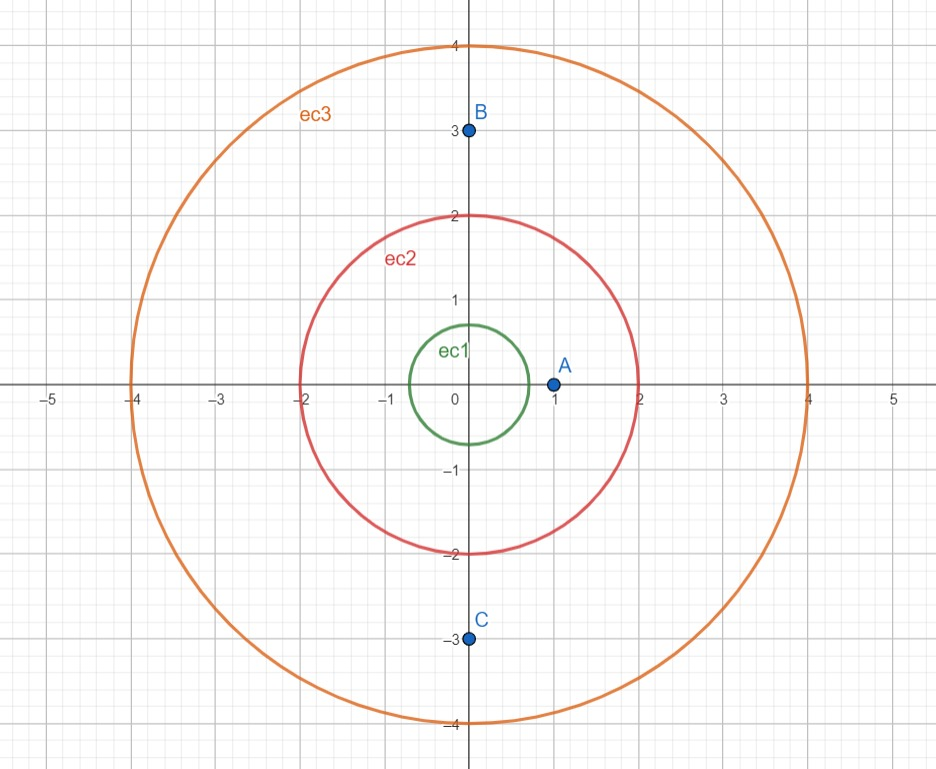
\includegraphics[width=\textwidth]{./Imagenes/foto1Ej5.jpeg}
    \end{minipage}\hfill
    \begin{minipage}{0.35\textwidth}
        \centering
        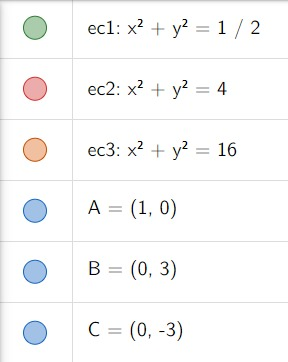
\includegraphics[width=\textwidth]{./Imagenes/foto2Ej5.jpeg}
    \end{minipage}
\end{figure}
       
Para calcular las integrales 1, 2 y 3 primero calculamos con las formulas de integracion de cauchy las integrales de las singularidades bajo la curva C. \\

\begin{align*}
I_{c1} &= \oint_{c}\frac{z+3j}{j(z - 1)^2(z-3j)(z+3j)} \, dz =\oint_{c}\frac{\frac{\cancel{z+3j}}{\cancel{(z+3j)}(z-1)^2}}{z-3j} \, dz\\[6pt]
&= \oint_{c}\frac{\frac{1}{(z-1)^2}(z-3j)}{z-3j} \, dz = 2\pi j \frac{1}{(3j-1)^2}\\[6pt]
I_{c2} &= \oint_{c}\frac{z+3j}{j(z - 1)^2(z-3j)(z+3j)} \, dz =\oint_{c}\frac{\frac{\cancel{z+3j}}{\cancel{(z+3j)}(z-1)^2}}{(z-1)^2} \, dz\\[6pt]
&= \oint_{c}\frac{\frac{1}{(z-3j)}}{(z-1)^2} \, dz = \frac{2\pi j}{(2-1)!} \left[ \frac{1}{z-3j} \right]_{z=1}^1= -\frac{2\pi j}{(1-3i)^2} \\[6pt]
I_{c3} &= \oint_{c}\frac{\cancel{z+3j}}{(z - 1)^2(z-3j)\cancel{(z+3j)}} \, dz=0 \\[6pt]
\end{align*}


Una vez obtenidas las curvas integrales se calculan las integrales 1, 2 y 3 haciendo un analisis de cuales singularidades estan bajo la curva $|z|=v$ y usando el teorema de deformacion de contorno: \\

\begin{align*}
I_1&=\oint_{|z|=\frac{1}{2}}f(z) \, dz= 0 \rightarrow \text{Por que no hay ninguna singularidad bajo la curva $|z|=\frac{1}{2}$}\\[6pt]
I_2&=\oint_{|z|=2}f(z) \, dz = I \oint_{c2} = - \frac{2 \pi j}{(1-3j)^2}\\[6pt]
    &\text{Por que bajo la curva $|z|=2$ esta la singularidad $z=1$}\\[12pt]
I_3&= \oint_{|z|=4}f(z) \, dz = I_{c2}+I_{c1}=2 \pi j \left( -\frac{1}{(1-3j)^2} + \frac{1}{(3j-1)^2} \right) = 0 \\[6pt]
\end{align*}
Otro metodo para hacerlos es mediante el teorema del residuo:\\
Primero se calulan los residuos de cada polo\\
\begin{align*}
&\text{Res}(f(z),3j)= \lim_{z \to 3j} \frac{\cancel{(z-3j)}\cancel{(z+3j)}}{(z-1)^2\cancel{(z-3j)}\cancel{(z+3j)}}= \lim_{z \to 3j} \frac{1}{(z-1)^2}=\frac{1}{(3j-1)^2} \\[6pt]
&\text{Res}(f(z),1)=\frac{1}{(2-1)!} \lim_{z \to 2} \frac{d}{\,dz} \left[ \cancel{(z-1)^2} \frac{\cancel{(z+3j)}}{\cancel{(z-1)^2}(z-3j) \cancel{(z+3j)}} \right]\\[6pt]
&\phantom{\text{Res}(f(z),1)}= \lim_{z \to 1} \frac{d}{\,dz} \left[ \frac{1}{z-3j} \right]= \frac{1}{(1-3j)^2}\\[6pt]
\end{align*}

Siguiendo la logica de que singularidad esta bajo la curva $|z|=r$ calculamos los integrales:

\begin{align*}
I_1&= \oint_{|z|=\frac{1}{2}}f(z) \, dz = 0 \rightarrow \text{no hay ninguna singularidad}\\[6pt]
I_2&= \oint_{|z|=2}f(z) \, dz = 2 \pi j \text{Res}\hspace{0.5cm}(f(z),1)= -\frac{2 \pi j}{(1-3j)^2}\\[6pt]
I_3&= \oint_{|z|=4}f(z) \, dz = 2 \pi j(\text{Res}(f(z),1)+\text{Res}(f(z),3j))\\[6pt]
&\phantom{I_3=\oint_{|z|=4}f(z) \, dz } =2\pi j \left( -\frac{1}{(1-3j)^2} + \frac{1}{(3j-1)^2} \right)\\[6pt]
&\phantom{I_3=\oint_{|z|=4}f(z) \, dz }=0\\[6pt]
\end{align*}

\textbf{d) Para evaluar las integrales del inciso, ¿en qué tenemos que concentrar nuestro análisis?}\\

Resolucion:\\
Para evaluar las integrales del inciso C tenemos que concentrar nuestro analisis en las singularidades de la funcion $f(z)$ con respecto a las curvas, cerradas en este caso.\\

\chapter{}%ejercicio 6

Con este ejercicio se busca que el estudiante obtenga información relevante de la serie de Laurent de una función en variable compleja.
Considerar la función de variable compleja $ f(z) = (z - 1)^2 e^\frac{1}{z - 1} $.\\[6pt]

\textbf{a)  Obtener la serie de Laurent de la función identificando claramente la Parte Analítica y la Parte Singular, esto es,}

$$ f(z) = \sum_{n=0}^{\infty} a_n(z - 1)^n + \sum_{n=1}^{\infty} b_n(z - 1)^{-n} $$

Para obtener la Serie de Laurent de esta funcion, partimos de la serie de McLaurin de $e^z$
$$e^z=\sum_{k=0}^{\infty}\frac{z^k}{k!}\quad,\quad k \in \mathbb{N}$$
Si realizamos la sustitucion:
$$e^\frac{1}{z - 1}=e^u \quad, \quad u=(z - 1)^{-1}$$
Entonces:
$$e^\frac{1}{z - 1}=\sum_{k=0}^{\infty}\frac{(z - 1)^{-k}}{k!}$$
Sustituyendo este resultado en nuestra funcion
$$f(z) = (z - 1)^2 \sum_{k=0}^{\infty}\frac{(z - 1)^{-k}}{k!}$$
$$f(z) = \sum_{k=0}^{\infty}\frac{(z - 1)^{-k+2}}{k!}$$
$$f(z) = \sum_{k=0}^{\infty}a_k(z - 1)^{-k+2}\qquad, \qquad a_k=\frac{1}{k!}$$

Observamos que el exponente $-k+2$
$$(-k+2) \geq 0 \quad \Leftrightarrow \quad k \leq 2$$
$$(-k+2) < 0 \quad \Leftrightarrow \quad k>2$$
Entonces podemos expresar la funcion como:
$$f(z) = \sum_{k=0}^{2}a_k(z - 1)^{-k+2} + \sum_{k=3}^{\infty}a_k(z - 1)^{-k+2}\qquad, \qquad a_k=\frac{1}{k!}$$
o lo que es igual:
$$f(z) = \underbrace{\sum_{n=0}^{2}a_n(z - 1)^{n}}_{\text{Parte Analitica}} + \underbrace{\sum_{n=1}^{\infty}b_n(z - 1)^{-n}}_{\text{Parte Singular}}
\qquad, \qquad a_n=\frac{1}{(2-n)!}\quad y \quad b_n=\frac{1}{(n+2)!}$$

\textbf{b)  Teniendo en cuenta la serie del inciso anterior clasificar la singularidad (evitable, polo, 
esencial) y calcular el residuo \( \text{Res}(f, z = 1) \).}

Ya que la parte singular de la serie de Laurent tiene infinitos terminos, podemos afirmar que la singularidad
en el punto $1+j0$ es esencial.

Por definicion, el residuo es el primer coeficiente de la Parte Singular de la serie de Laurent, por ende:
$$\text{Res}(f, z = 1) = b_1=\frac{1}{(1+2)!} = \frac{1}{6}$$

\textbf{c)  Valuar las siguientes integrales:}

$$ I_1 = \oint_{|z| =\frac{1}{2}} f(z) \, dz; \quad I_2 = \oint_{|z| = 2} f(z) \, dz; \quad I_3 = \oint_{|z| = 4} f(z) \, dz $$

Como que no hay singularidades dentro de la curva $|z|=\frac{1}{2}$
$$\oint_{|z| = 1/2} f(z) \, dz = 0$$

Para la segunda integral, aplicando teorema del residuo
$$\oint_{|z| = 2} f(z) \, dz = 2\pi j \text{Res}(f, z = 1) = 2\pi j\frac{1}{6}=\frac{1}{3}\pi j$$

De igual forma para la tercer integral
$$\oint_{|z| = 4} f(z) \, dz = 2\pi j \text{Res}(f, z = 1) =\frac{1}{3}\pi j$$\\

\textbf{d)  Teniendo en cuenta el inciso anterior podemos afirmar que:}

$$ I_r = \oint_{|z| = r} f(z) \, dz = I_1, \text{ para todo } 0 < r < 1 $$ 
Ya que cualquier curva en este intervalo no va a incluir al unico punto singular que tiene nuestra funcion

Y:
$$ I_r = \oint_{|z| = r} f(z) \, dz = I_2, \text{ para todo } r > 1 $$ 
De manera opuesta, todas estas curvas van a incluir al unico punto singular de la funcion

\chapter{}%ejercicio 7

    Con este ejercicio se busca que el estudiante calcule integrales del Análisis I empleando la variable compleja de forma metodológica.\\

Calcular el área bajo la curva\\


\begin{figure}[h] % Aquí comienza el ambiente de figura
    \centering % Centrar la imagen
    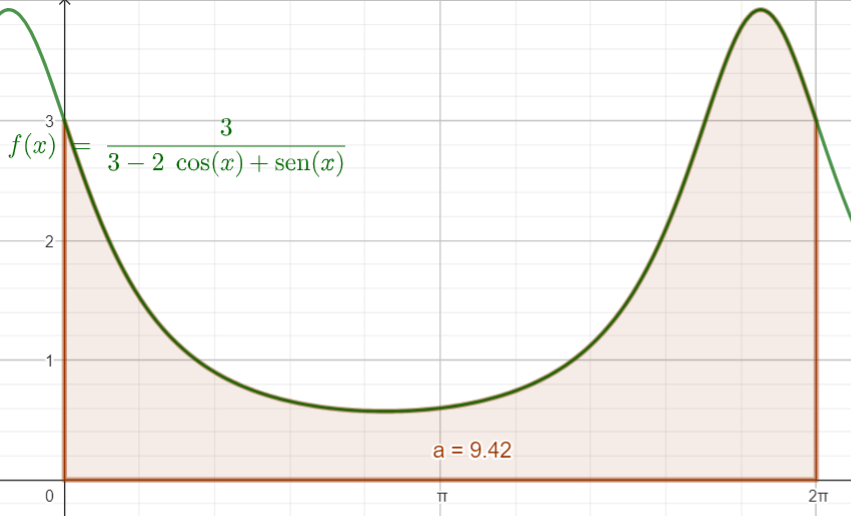
\includegraphics[width=0.65\textwidth]{./Imagenes/foto1Ej7.png} % Insertar la imagen
\end{figure}

$a = \int_{0}^{2\pi} \frac{3}{3 - 2\cos(x) + \sin(x)} \, dx$\\[6pt]

siguiendo los siguientes pasos:\\[6pt]

\textbf{a)  Defina $z = e^{x}$ y con ello consiga las siguientes igualdades:}\\[6pt]

$dx = \frac{dz}{jz}; \quad \cos(x) = \frac{z^{2} + 1}{2z}; \quad \sin(x) = \frac{z^{2} - 1}{2jz}$\\[6pt]

\textbf{b)  Realizar una sustitución para obtener una función racional en la variable \( z \):}

$$ f(x) \, dx = \frac{3}{3 - 2\int \left( \frac{z^{2} + 1}{2z} \right) \, dz + \int \left( \frac{z^{2} - 1}{2jz} \right) \, dz} \cdot \frac{dz}{jz} = R(z) \, dz $$ 

Y con ello, se valida la igualdad:

$$ \int_{0}^{2\pi} f(x) \, dx = \oint_{|z|=1} R(z) \, dz$$ 


\textbf{c)  Finalmente, clasificar todas las singularidades de la función racional $R(z)$ y usar el teorema del residuo para calcular el lado derecho de la integral formulada en el inciso anterior.}


\end{document}

